\documentclass[a0]{tumposter}

\usepackage[english]{babel}

\usepackage{blindtext}

\usepackage{multicol}
\usepackage{amsmath}
\usepackage{graphicx}

% for printing fontsizes
\usepackage{printlen}
\uselengthunit{mm}

\input{preamble.tex}

\usepackage[utf8]{inputenc}

\title{
	Early Classification for Agricultural Monitoring \\ from Satellite Time Series
	}
	
\author{
	Marc Rußwurm\footnotemark[1], Romain Tavenard\footnotemark[2], Sébastien Lefèvre\footnotemark[2], Marcoa Körner\footnotemark[1]
	}

\header{
	Remote Sensing Technology \\
	TUM Department of Civil, Geo and Environmental Engineering \\
	Technical University of Munich
	}
	
\begin{document}
\maketitle

\renewcommand{\subsection}[1]{\textbf{#1}}

\begin{minipage}[t]{.65\textwidth}
	
	\section{Objective}
	
	
	\begin{tikzpicture}[scale=16.8]
	\node[label={[name=sat,text height=1.5ex,text depth=.25ex]Satellite Data}, anchor=north](x) at (-1,0){$\M{X} = (\V{x}_0, \V{x}_1, \dots , \V{x}_T)$};
	\node[below=of x, label={[yshift=1.3em, xshift=1.8em, font=\tiny, text=white]below:ESA Sentinel 2 Satellite}](s2){\includegraphics[width=11cm]{images/sentinel2}};
	
	
	\node[below=0em of s2, text width=11cm](eqbox){
		\small
		\begin{itemize}
			\item collected at regular temporal intervals of 2-3 days
			\item measurements of 13 spectral bands
			\item data available globalls
		\end{itemize} 
	};
	
	\node[label={[name=cm,text height=1.5ex,text depth=.25ex]{Early} {Classification} Model}, anchor=north](f) at (0,0){ $\yhat_t, {\deltat} = f(\xuptot)$};
	\node[below=0em of f, text width=13cm, font=\small](info){
		\begin{description}
		
		\item[$\xuptot$] observation until $t$  \\
		\item[$\yhat_t$] class prediction scores \\
		\item[$\deltat$] probability of stopping.
		
		\end{description}
		
	};
%	\node[below=of f](example){\input{images/example.tikz}};
	\node[circle, below=of info, text width=11cm, fill=tumbluedark, text=white](example){Classifying a \\ satellite time series \\ {\color{tumbluelight}\textbf{accurately}} \color{white} as {\color{ecolor}\textbf{early}} \color{white} as possible};
	
	
	\node[label={[name=ctm,text height=1.5ex,text depth=.25ex]Crop Type Labels}, anchor=north](y) at (1,0){
		$\V{y} = \small (y_\text{corn}, y_\text{barley}, \dots) \in \mathbb{R}^{13}$
	};
	\node[below=of y, label=below:crop type labels](labels){\includegraphics[width=11cm]{images/parcels}};
	\node[below=of labels, text width=11cm](lbls){
		\small
		\begin{itemize}\setlength\itemsep{.1em}
		\item European Common Agricultural Policy (CAP)
		\item collected yearly in entire Europe
%		\item slowly made publicly available
%		\item today, gathered on a national basis
%		\item in future harmonized within Europe's INSPIRE directive
		\end{itemize}
	};
	
	\draw[very thick, -{Stealth[scale=.5]}, tumblue] (x) -- (f);
	\draw[very thick, -{Stealth[scale=.5]}, tumblue] (f) -- (y);
	
	\coordinate(bottomleftcolumn) at (example.south -| s2);
	\coordinate(bottomrightcolumn) at (example.south -| lbls);
	
	\scoped[on background layer]
	{
		\node[fit=(ctm)(lbls)(bottomrightcolumn), fill=tumbluelight!20, inner sep=1em, rounded corners]{};
		\node[fit=(f)(example)(cm), fill=tumorange!20, inner sep=1em, rounded corners]{};
		\node[fit=(sat)(eqbox)(bottomleftcolumn), fill=tumbluelight!20, inner sep=1em, rounded corners]{};
	}	
	
	\end{tikzpicture}
	
	
	\section{Method}
	
	Based on previous work (Rußwurm et al., 2019) applied to crop type mapping from remote sensing data.
	
	%A network output to indicate a probability of stopping $\deltat$
	
	\begin{minipage}[t]{.49\textwidth}
		\subsection{Mechanism}
		
		\newcommand{\backpropstoppingrulefull}{
\tikzsetnextfilename{backprop_stopping_rule}
\begin{tikzpicture}[node distance=1em and 1em]
\node[](x0){$x_t$};
\node[rnn, below=of x0](h0){$h_t$};  %$\theta_\text{rnn}$};
\node[below right= 2em and 1em of h0](y0){$\yhat_t$};
\node[rnn, left=2em of h0,draw=lightgray](hprev){};
\node[rnn, right=2em of h0,draw=lightgray](hnext){};
\node[below left= 2em and 1em of h0](d0){$\delta_t$};

\node[loss, below=of y0](L0){$\mathcal{L}_c (\xuptot, y)$};
%\node[right=of L0](t0){$\V{y}_t$};
\draw[-stealth, grad] (y0) -- (L0);
%\draw[-stealth, grad] (t0) -- (L0);

\draw[infer] (x0) -- (h0);
\draw[infer,draw=lightgray] (hprev) -- (h0);
\draw[infer,draw=lightgray] (h0) -- (hnext);
\draw[infer] (h0) -- (y0) node[midway,right, text=black](wc){$\theta_{cl}$};
\draw[infer] (h0) -- (d0) node[midway,left, text=black](wd){$\theta_{\delta}$};

\draw[-stealth, grad] (L0) to [bend right=30] node[near end, right, text=colortrain]{$\frac{\partial\mathcal{L}}{\partial\theta_\text{cl}}$}
(wc);

\node[below=of d0](pt){$P(t)$};
\node[below=8em of h0, loss](L){$\mathcal{L}_t(\xuptot, y ; \alpha)$}; % = P(t)\mathcal{L}_c (\xuptot, y)$};

\node[left=.5em of pt](budget){$\mathcal{B}_{t-1}$};

\draw[infer] (L0) -- (L);
\draw[infer] (d0) -- (pt);
\draw[infer] (pt) -- (L);
\draw[infer] (budget) -- (pt);

\draw[-stealth, grad] (L) to [bend right=30] node[midway, right, text=colortrain]{$\frac{\partial\mathcal{L}}{\partial\mathcal{L}_c}$}(L0);

\draw[-stealth, grad] (L) to [bend left=30] node[midway, left, text=colortrain]{$\frac{\partial\mathcal{L}}{\partial P(t)}$}(pt);

\draw[-stealth, grad] (pt) to [bend left=30] node[midway, left, text=colortrain]{$\frac{\partial\mathcal{L}}{\partial \theta_{\delta}}$}(wd);

\end{tikzpicture}
}
		\backpropstoppingrulefull
		
%	\begin{tikzpicture}
%		\node[fill=tumbluelight!20, rounded corners](a) at (0,0){
%						\newcommand{\backpropstoppingrulefull}{
\tikzsetnextfilename{backprop_stopping_rule}
\begin{tikzpicture}[node distance=1em and 1em]
\node[](x0){$x_t$};
\node[rnn, below=of x0](h0){$h_t$};  %$\theta_\text{rnn}$};
\node[below right= 2em and 1em of h0](y0){$\yhat_t$};
\node[rnn, left=2em of h0,draw=lightgray](hprev){};
\node[rnn, right=2em of h0,draw=lightgray](hnext){};
\node[below left= 2em and 1em of h0](d0){$\delta_t$};

\node[loss, below=of y0](L0){$\mathcal{L}_c (\xuptot, y)$};
%\node[right=of L0](t0){$\V{y}_t$};
\draw[-stealth, grad] (y0) -- (L0);
%\draw[-stealth, grad] (t0) -- (L0);

\draw[infer] (x0) -- (h0);
\draw[infer,draw=lightgray] (hprev) -- (h0);
\draw[infer,draw=lightgray] (h0) -- (hnext);
\draw[infer] (h0) -- (y0) node[midway,right, text=black](wc){$\theta_{cl}$};
\draw[infer] (h0) -- (d0) node[midway,left, text=black](wd){$\theta_{\delta}$};

\draw[-stealth, grad] (L0) to [bend right=30] node[near end, right, text=colortrain]{$\frac{\partial\mathcal{L}}{\partial\theta_\text{cl}}$}
(wc);

\node[below=of d0](pt){$P(t)$};
\node[below=8em of h0, loss](L){$\mathcal{L}_t(\xuptot, y ; \alpha)$}; % = P(t)\mathcal{L}_c (\xuptot, y)$};

\node[left=.5em of pt](budget){$\mathcal{B}_{t-1}$};

\draw[infer] (L0) -- (L);
\draw[infer] (d0) -- (pt);
\draw[infer] (pt) -- (L);
\draw[infer] (budget) -- (pt);

\draw[-stealth, grad] (L) to [bend right=30] node[midway, right, text=colortrain]{$\frac{\partial\mathcal{L}}{\partial\mathcal{L}_c}$}(L0);

\draw[-stealth, grad] (L) to [bend left=30] node[midway, left, text=colortrain]{$\frac{\partial\mathcal{L}}{\partial P(t)}$}(pt);

\draw[-stealth, grad] (pt) to [bend left=30] node[midway, left, text=colortrain]{$\frac{\partial\mathcal{L}}{\partial \theta_{\delta}}$}(wd);

\end{tikzpicture}
}
%						\backpropstoppingrulefull
%					};
%		\node[right=of a]{\input{images/qualitative_example.tikz}};
%	\end{tikzpicture}
%	\vspace{-10em}

%	probability of not having classified before (known at training time)
%	$$P(t) = \deltat \cdot \prod_{\tau=0}^{t-1} 1 - p_\tau$$

	

	\end{minipage}
	\begin{minipage}[t]{.49\textwidth}
		
	
	\subsection{Loss function}
	
	composite loss function
	$$\mathcal{L}(\V{x}, \V{y}) = \sum_{t=0}^T P(t;\deltauptot) \mathcal{L}_t(\xuptot, \V{y})$$
	
	
	A Loss function including accuracy and earliness
	
	\begin{tikzpicture}[node distance=-.5em, draw=tumbluelight, rounded corners]
	
	%	\node(allloss){$\mathcal{L}(\V{x}, \V{y}) = \sum_{t=0}^T P(t;\deltauptot) \mathcal{L}_t(\xuptot, \V{y})$};
	%	
	\node(loss){$\mathcal{L}_t(\xuptot, \V{y})$};
	\node[right=of loss](equals){$=$};
	\node[right=of equals, fill=accuracycolor!20, rounded corners, label={[font=\small]Classification Loss}](classificationloss){$\alpha \mathcal{L}_c (\xuptot, \V{y})$};
	\node[right=of classificationloss](minus){$-$};
	\node[right=of minus, fill=earlinesscolor!20, rounded corners, label={[font=\small]Earliness Reward}](earlinessreward){$(1 - \alpha)\mathcal{R}_e(t, \ycorrect_t)$};
	
	\node[below=1em of classificationloss, text width=10cm, xshift=-4em](clossexp){$\mathcal{L}_c = -\log(\ycorrect_t)$ \\
		\vspace{.5em} 
		\tiny
		cross entropy loss for accurate classifications \par};
	
	\node[below=1em of earlinessreward, text width=13cm, xshift=-2em](erewardexp){$\mathcal{R}_e(t, \ycorrect_t) = \ycorrect_t \left(1 - \frac{t}{T}\right)$ \\
		\vspace{.5em}
		\tiny
		reduces loss for earlier classifications $1-\frac{t}{T}$ if the correct class $\ycorrect_t$ has been predicted with a high score \par};
	
	\draw[thick] (classificationloss) -- (clossexp);
	\draw[thick] (earlinessreward) -- (erewardexp);
	\end{tikzpicture}
	
	
	\end{minipage}

	{\tiny 
	Rußwurm, M., Lefèvre, S., Courty, N., Emonet, R., Körner, M., and Tavenard, R. End-to-end learning for early classification of time series. arXiv preprint arXiv:1901.10681, 2019.
	\par
	}

	
	\section{Application}
	
	\begin{minipage}[t]{.5\textwidth}
	\subsection{Agriculture}
	
	\small
	
	\vspace{1em}
	
		\textbf{Early Crop Detection}
		\begin{itemize}
			\item early assessment of cultivated crops
			\item basis for early crop yield estimation
		\end{itemize}
		\vspace{.3em}
		
		\textbf{Extraction of Crop Phenology}
		\begin{itemize}
			\item extraction of vegetation specific events 
			\item monitoring time of classification
			\item regional or temporal variations
		\end{itemize}
		\vspace{.3em}
		
		\textbf{Generalization}
		\begin{itemize}
			\item end-to-end trainable
			\item applicable globally
			\item no region-specific expert knowledge
		\end{itemize}
	
	\end{minipage}
	\begin{minipage}[t]{.66\textwidth}
	\subsection{Dataset and Area of Interest} \par
	\begin{minipage}{.49\textwidth}
		\small
		\vspace{1em}
		Hollfeld region Bavaria
		\begin{itemize}
			\item 49k field parcels
			\item 6 main crop types
			\item covering 40 by 30 km
			\item central germany
		\end{itemize}
		
		\vspace{1em}
	
		\tiny Challenge: Class imbalance \par
		\input{images/partition_histograms.tikz}
%		\vspace{-4em}\includegraphics[width=.3\textwidth]{images/holl.pdf}
	\end{minipage}
	\begin{minipage}{.33\textwidth}
%		\input{images/partition_histograms.tikz}
		\tiny {\color{tumblue}regions with labels} and \\ {\color{tumorange} location of dataset} \par
		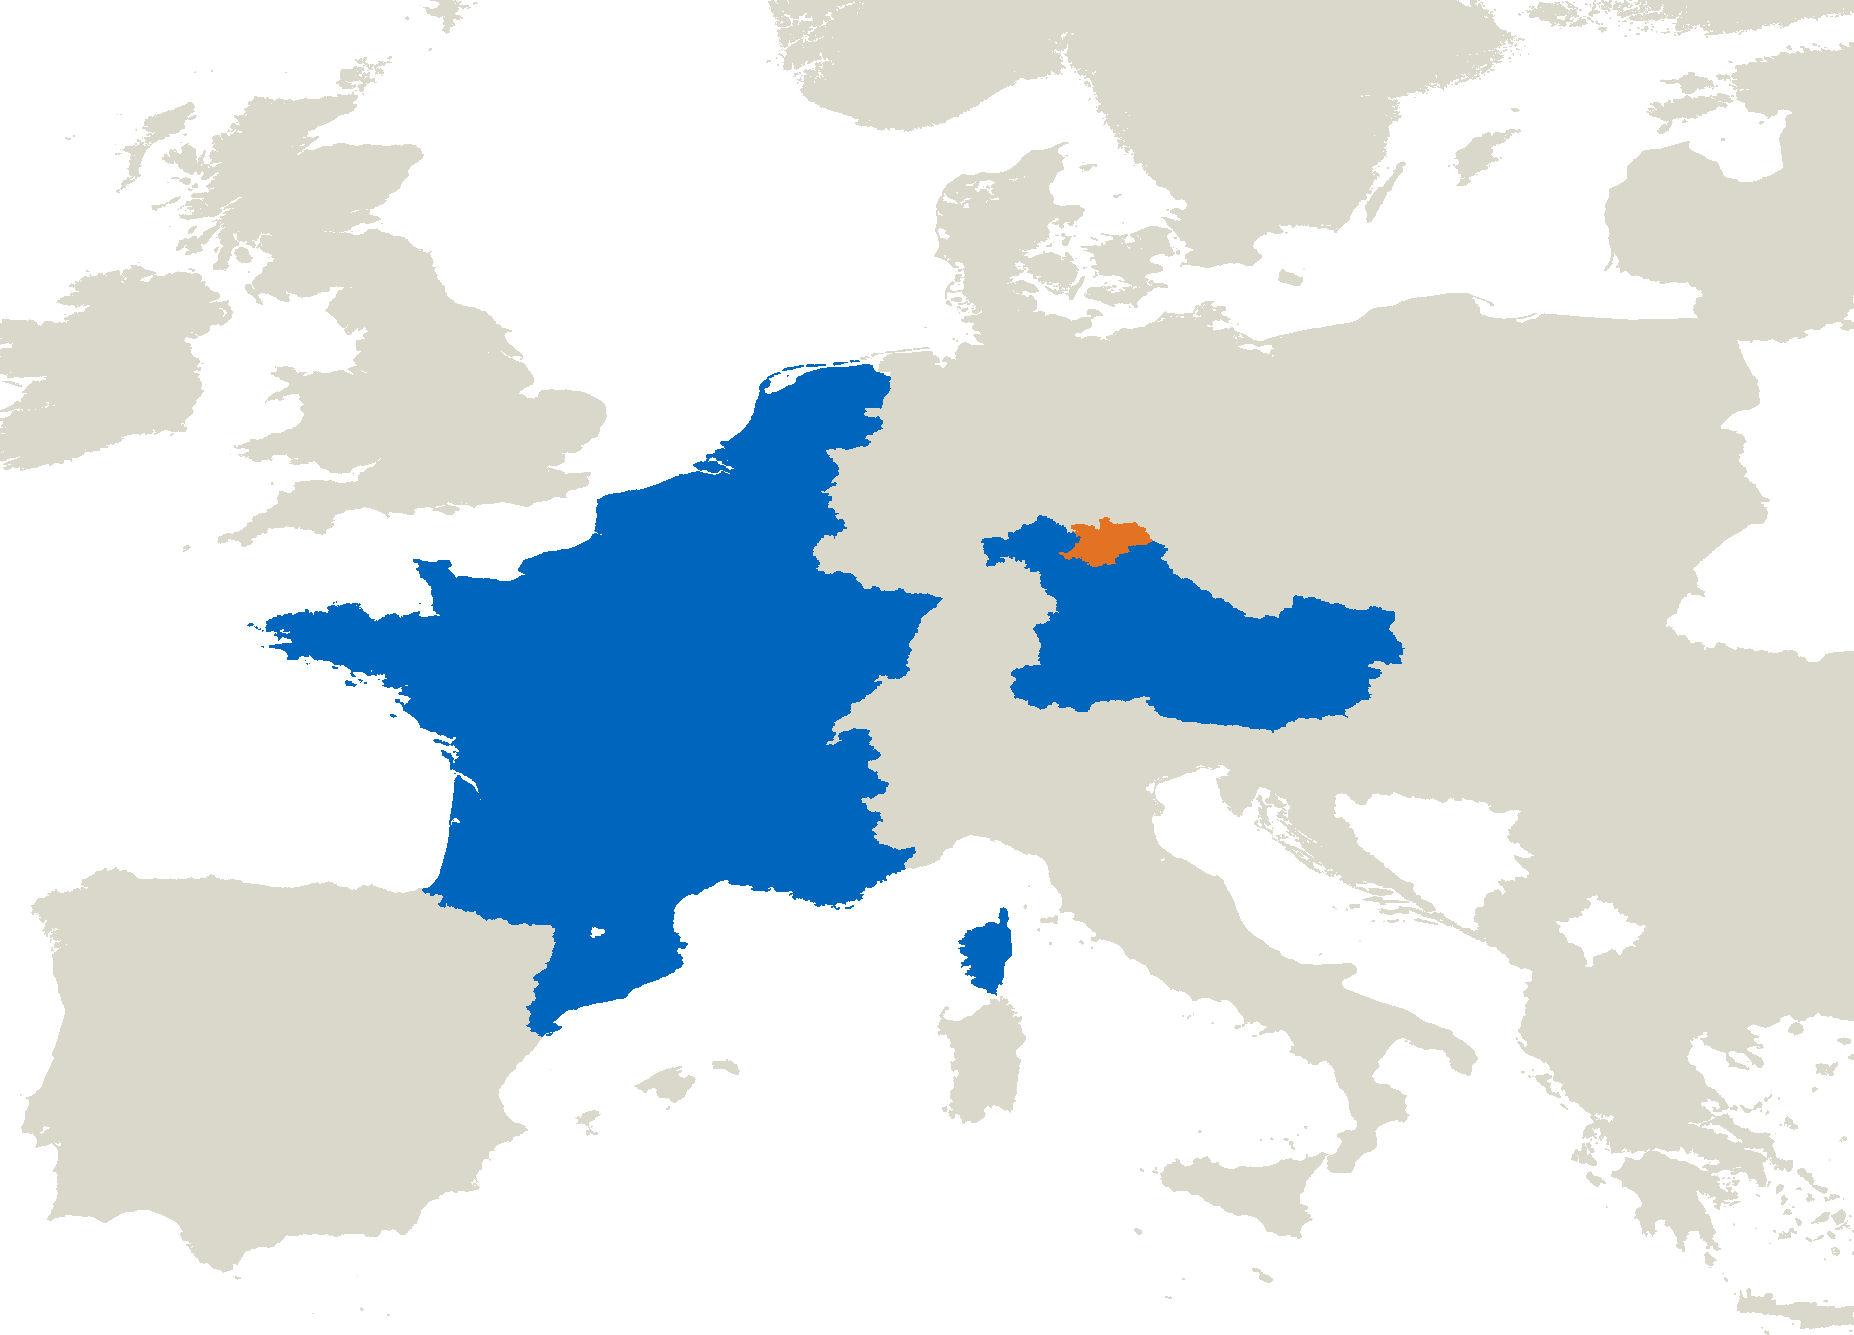
\includegraphics[width=.9\textwidth]{images/oberfrankenineurope.pdf}
		 
		 \tiny partition in {\color{traincolor} train}, {\color{validcolor} validation}, and {\color{evalcolor} evaluation} \par
		\includegraphics[width=.9\textwidth]{images/holl.pdf}
	\end{minipage}
	
	\end{minipage}

\end{minipage}
\hfill
\begin{minipage}[t]{.32\textwidth}
	\section{Results}
	
	\subsection{Qualitative Example}
	
	\input{images/example.tikz}
	
	\subsection{Losses during Training}
	
	\small
	
	The combined loss $L_t$, as well as earliness $L_e$ and accuracy $L_e$ losses during training.
	
	%\newcommand{\figearlyreward}{
\def\datapath{images/logs/data/early_reward_p2/classes}
\tikzsetnextfilename{loss-accuracyplots}
\begin{tikzpicture}
	\begin{groupplot}[
	group style = {
		group size = 1 by 2,
		x descriptions at=edge bottom,
		vertical sep=1em},
	no markers,
	height=4cm,
%	legend style={at={(0.03,0.5)},anchor=west},
	width=.9\textwidth,
	xlabel=epochs,
	xlabel style={yshift=-.5em},
	ymajorgrids,
	xtick={0, 10,...,100},
	ylabel style={yshift=2.3em}
 	]
	\nextgroupplot[thin, legend columns=3, ylabel=loss]

	\addplot[tumblack] table [x=epoch, y=loss, col sep=comma] {\datapath/log_earliness_test.csv};
	
	\addplot[accuracycolor] table [x=epoch, y=loss_classification, col sep=comma] {\datapath/log_earliness_test.csv};
	
	\addplot[earlinesscolor] table [x=epoch, y=earliness_reward, col sep=comma] {\datapath/log_earliness_test.csv};
	
%	\legend{total loss (eval), classification loss (eval), earliness reward (eval)}
%	
	\legend{$\mathcal{L}_\text{t}$, $\mathcal{L}_\text{c}$, $\mathcal{R}_\text{e}$}
	
	
	
	\nextgroupplot[thin,
		legend columns=2, 
		legend pos=south east,
		ytick={0,0.5,1},
		yticklabels={
			0 ({\color{earlinesscolor} jan}),
			0.5 ({\color{earlinesscolor} jun}),
			1 ({\color{earlinesscolor} dec})},
		ylabel={\color{tumorange}accuracy}/\color{tumblue}$\meantstop$]
	\addplot[accuracycolor] table [x=epoch, y=accuracy, col sep=comma] {\datapath/log_earliness_test.csv};
	\addplot[earlinesscolor] table [x=epoch, y=earliness, col sep=comma] {\datapath/log_earliness_test.csv};

	\legend{accuracy,$\meantstop$}
	
	\end{groupplot}
\end{tikzpicture}
%
%}
	\figearlyreward
	
	\subsection{Stopping rules learned for each Class}
	
	\def\datapath{images/logs/data/early_reward_p2/classes}

\tikzsetnextfilename{trainingstoppingclasses}
\begin{tikzpicture}
	\begin{groupplot}[
	group style = {
		group size = 1 by 2,
		x descriptions at=edge bottom,
		vertical sep=.75em},
	title style={
		font=\sffamily\scriptsize,
		at={(0,1.1)},
		anchor=north west
	},
	ymajorgrids,
	no markers,
	height=5cm,
	legend style={at={(0.5,1)},anchor=south},
	width=.9\textwidth,
	xlabel=epochs,
	ymax=1.1,
	ymin=0.3,
	ylabel=$\tstop$,
	ylabel style={yshift=1em},
	xlabel style={yshift=-.5em},
	ytick={0,0.25,0.5,0.75,1},
	xtick={0, 10,...,100},
	yticklabels={jan,apr,jun,sep,dec}
	]
	\nextgroupplot[title=meadows, legend columns=3]
	\addplot[meancolor] table [x=epoch, y=meadows, col sep=comma] {\datapath/mean.csv};
	\addplot[mediancolor] table [x=epoch, y=meadows, col sep=comma] {\datapath/median.csv};
	\addplot+[name path=upper, draw=none,forget plot] table [x=epoch, y=meadows, col sep=comma] {\datapath/mean+std.csv};
	\addplot+[name path=lower, draw=none,forget plot] table [x=epoch, y=meadows, col sep=comma] {\datapath/mean-std.csv};
	\addplot[stdcolor] fill between[of=lower and upper];
	
	\legend{mean, median, mean $\mp$ std}
	
	\nextgroupplot[title=winter barley]
	\addplot[meancolor] table [x=epoch, y=winter barley, col sep=comma] {\datapath/mean.csv};
	\addplot[mediancolor] table [x=epoch, y=winter barley, col sep=comma] {\datapath/median.csv};
	\addplot+[name path=upper, draw=none] table [x=epoch, y=winter barley, col sep=comma] {\datapath/mean+std.csv};
	\addplot+[name path=lower, draw=none] table [x=epoch, y=winter barley, col sep=comma] {\datapath/mean-std.csv};
	\addplot[stdcolor] fill between[of=lower and upper];
	
%	\nextgroupplot[title=corn]
%	\addplot[meancolor] table [x=epoch, y=corn, col sep=comma] {\datapath/mean.csv};
%	\addplot[mediancolor] table [x=epoch, y=corn, col sep=comma] {\datapath/median.csv};
%	\addplot+[name path=upper, draw=none] table [x=epoch, y=corn, col sep=comma] {\datapath/mean+std.csv};
%	\addplot+[name path=lower, draw=none] table [x=epoch, y=corn, col sep=comma] {\datapath/mean-std.csv};
%	\addplot[stdcolor] fill between[of=lower and upper];
%	
%	\nextgroupplot[title=winter wheat]
%	\addplot[meancolor] table [x=epoch, y=winter wheat, col sep=comma] {\datapath/mean.csv};
%	\addplot[mediancolor] table [x=epoch, y=winter wheat, col sep=comma] {\datapath/median.csv};
%	\addplot+[name path=upper, draw=none] table [x=epoch, y=winter wheat, col sep=comma] {\datapath/mean+std.csv};
%	\addplot+[name path=lower, draw=none] table [x=epoch, y=winter wheat, col sep=comma] {\datapath/mean-std.csv};
%	\addplot[stdcolor] fill between[of=lower and upper];
%	
%	\nextgroupplot[title=summer barley]
%	\addplot[meancolor] table [x=epoch, y=summer barley, col sep=comma] {\datapath/mean.csv};
%	\addplot[mediancolor] table [x=epoch, y=summer barley, col sep=comma] {\datapath/median.csv};
%	\addplot+[name path=upper, draw=none] table [x=epoch, y=summer barley, col sep=comma] {\datapath/mean+std.csv};
%	\addplot+[name path=lower, draw=none] table [x=epoch, y=summer barley, col sep=comma] {\datapath/mean-std.csv};
%	\addplot[stdcolor] fill between[of=lower and upper];
%	
%	\nextgroupplot[title=clover]
%	\addplot[meancolor] table [x=epoch, y=clover, col sep=comma] {\datapath/mean.csv};
%	\addplot[mediancolor] table [x=epoch, y=clover, col sep=comma] {\datapath/median.csv};
%	\addplot+[name path=upper, draw=none] table [x=epoch, y=clover, col sep=comma] {\datapath/mean+std.csv};
%	\addplot+[name path=lower, draw=none] table [x=epoch, y=clover, col sep=comma] {\datapath/mean-std.csv};
%	\addplot[stdcolor] fill between[of=lower and upper];
%	
%	\nextgroupplot[title=winter triticale]
%	\addplot[meancolor] table [x=epoch, y=winter triticale, col sep=comma] {\datapath/mean.csv};
%	\addplot[mediancolor] table [x=epoch, y=winter triticale, col sep=comma] {\datapath/median.csv};
%	\addplot+[name path=upper, draw=none,forget plot] table [x=epoch, y=winter triticale, col sep=comma] {\datapath/mean+std.csv};
%	\addplot+[name path=lower, draw=none,forget plot] table [x=epoch, y=winter triticale, col sep=comma] {\datapath/mean-std.csv};
%	\addplot[stdcolor] fill between[of=lower and upper];

	
	\end{groupplot}
	\end{tikzpicture}
	
	\subsection{Balancing Earliness and Accuracy} \par
	\begin{table}
		
		\scriptsize
		\hspace{0em}\begin{tabular}{lcccccc}
			\toprule\small
			\textbf{$\alpha$} & accuracy & $\meantstop$  & precision & recall & $f_1$ & $\kappa$ \\
			\cmidrule(lr){0-0}\cmidrule(lr){1-1}\cmidrule(lr){2-2}\cmidrule(lr){3-3}\cmidrule(lr){4-4}\cmidrule(lr){5-5}\cmidrule(lr){6-6}\cmidrule(lr){7-7}
			.0 & .25 $\pm$ .22 & .10 $\pm$ .17 & .19 $\pm$ .20 & .25 $\pm$ .17 & .16 $\pm$ .20 & .12 $\pm$ .19 \\
			.2 & .81 $\pm$ .03 & .40 $\pm$ .02 & .70 $\pm$ .01 & .74 $\pm$ .01 & .71 $\pm$ .01 & .71 $\pm$ .04 \\
			.4 & .80 $\pm$ .09 & .47 $\pm$ .03 & .71 $\pm$ .02 & .74 $\pm$ .01 & .71 $\pm$ .02 & .71 $\pm$ .10 \\
			.6 & .85 $\pm$ .02 & .88 $\pm$ .07 & .73 $\pm$ .04 & .74 $\pm$ .03 & .73 $\pm$ .03 & .77 $\pm$ .03 \\
			.8 & .84 $\pm$ .01 & .93 $\pm$ .05 & .72 $\pm$ .02 & .75 $\pm$ .01 & .73 $\pm$ .02 & .76 $\pm$ .02 \\
			1.0 & .83 $\pm$ .03 & 1.00 $\pm$ .00 & .72 $\pm$ .03 & .75 $\pm$ .01 & .72 $\pm$ .03 & .75 $\pm$ .04 \\
			\bottomrule
		\end{tabular}
	
		experiments varying the trade-off factor $\alpha$ and observing the achieved earliness and accuracy.
	
		%	\caption{Varying the weighting factor $\alpha$ for \emph{early reward} loss formulation (\cref{sec:earlynessreward}).}
		%	\label{tab:alpha}
		
	\end{table}
	
	
	\subsection{Extracting Vegetation Characteristics}
	
	Stopping time grouped per crop category 
	\input{images/classboxplots.tikz}
	
%	\tiny
%	\bibliographystyle{icml2019}
%	\bibliography{bib/references.bib}
%	
	
\end{minipage}

\begin{footer}
	\begin{minipage}{.33\textwidth}
		\textbf{Technical University of Munich}\footnotemark[1]\\
		TUM Department of Civil, Geo and Env. Engineering \\
		Remote Sensing Technology \\
		Arcisstr. 21, 80333 Munich, Germany
	\end{minipage}
	\begin{minipage}{.33\textwidth}
		\textbf{IRISA-Obelix}\footnotemark[2]\\
		Université Bretagne Sud \\
		IRISA, UMR 6074 CNRS \\
		Campus de Tohannic, 56000 Vannes, France
		
	\end{minipage}
	\begin{minipage}{.23\textwidth}
		\textbf{Data \& Code} \\
		%		\vspace{1em}
		{https://github.com/rtavenar/early\_rnn} \\
		{https://twitter.com/MarcCoru} \\
		www.lmf.bgu.tum.de/vision
	\end{minipage}
	\begin{minipage}{.10\textwidth}
		\hfill\includegraphics[width=5cm]{images/qr-code}\\
		
	\end{minipage}
	
	
\end{footer}

\end{document}